% Преамбула

% определяем формат страницы и тип документа ( А4, 12 пунктов, статья)
\documentclass[a4paper,12pt]{article}

% Задаём отступы и межстрочный интервал
\usepackage[top=2cm,bottom=2cm,left=3cm,right=2cm,marginparwidth=1.75cm]{geometry}

% подключаем пакеты расширения LaTeX
\usepackage{cmap}					% поиск в PDF
\usepackage[T2A]{fontenc}			% кодировка
\usepackage[utf8]{inputenc}			% кодировка исходного текста
\usepackage[english,russian]{babel}	% Русский язык и переносы
\usepackage{indentfirst} 			% красная строка
\frenchspacing						
\usepackage[utf8]{inputenc}			% кодировка	
\usepackage[T1]{fontenc}			

% полезные пакетики
\usepackage{amsmath} 									% для продвинутых формул
\usepackage{graphicx}									% для графиков
\usepackage[colorinlistoftodos]{todonotes}				% для пометок
\usepackage[colorlinks=true, allcolors=blue]{hyperref}	% расширенная поддержка гиперссылок
\usepackage{comment}									% многострочные комментарии
\usepackage{ulem}										% зачёркнутый текст
\usepackage{xcolor}										% цветной текст
\usepackage{color}										% цветной код
\usepackage{listings}									% отображает блоки кода

% настройка пакета подсветки исходного кода (не совсем рабочий)
\lstloadlanguages{ [LaTeX ] TeX, bash , Fortran , Perl ,C++,make} 
\lstset{ 			language =[LaTeX ] TeX,		 % выбираем язык по умолчанию
                    extendedchars=true , 		 % включаем не латиницу (не работает)
                    escapechar =| , 			 % |«выпадаем» в LATEX|
                    frame=tb , 					 % рамка сверху и снизу ( lr - слева, справа )
                    commentstyle=\itshape , 	 % шрифт для комментариев
                    stringstyle =\bfseries }	 % шрифт для строк



\author{ООО "ЛМП"} % Вводим своё имя
\title{Гироскопирование с МГ-25}  % Заголовок
\date{\today} % установка даты

\begin{document}
\maketitle
% \begin{abstract}
% Your abstract.
% \end{abstract}

\section{Ошибки прибора МГ-25}
\subsection{Оценка ошибки смещения нуля при изменении температуры по шагам}
Были проведены эксперименты с охлаждением устройства МГ-25 с задержкой в точках 70, 50, 30, 10, -10, и -30 градусов цельсия и последующим нагревом и задержкой в точках -40, -20, 0, 20, 40, 60 и 80 градусов. В каждой точке данные акселерометров и гировскопов были усреднены и построены графики изменения смещения нуля в температуре. На рисунке ~\ref{fig:gyro_bias_steps} представлены графики смещения нуля гироскопов в температуре. На рисунках ~\ref{fig:Ax_accel}, ~\ref{fig:Ay_accel} и ~\ref{fig:Az_accel} представлены графики смещения нуля акселерометров в температуре.

\begin{figure}
\centering
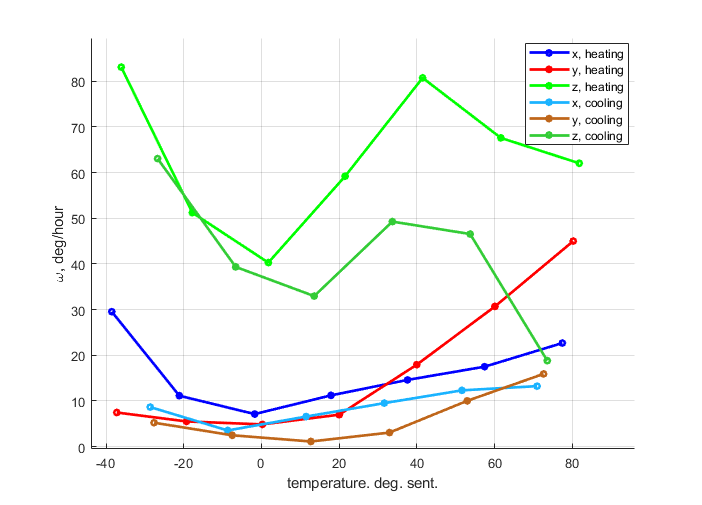
\includegraphics[width=0.9\textwidth]{gyro_bias_steps3.png} 
\caption{\label{fig:gyro_bias_steps} Смещения нуля гироскопов в температуре.}
\end{figure}
\begin{figure}
\centering
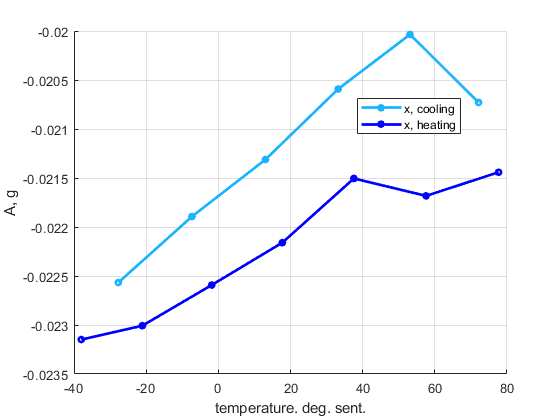
\includegraphics[width=0.9\textwidth]{Ax_accel.png} 
\caption{\label{fig:Ax_accel} Смещения нуля оси Х акселерометра в температуре.}
\end{figure}
\begin{figure}
\centering
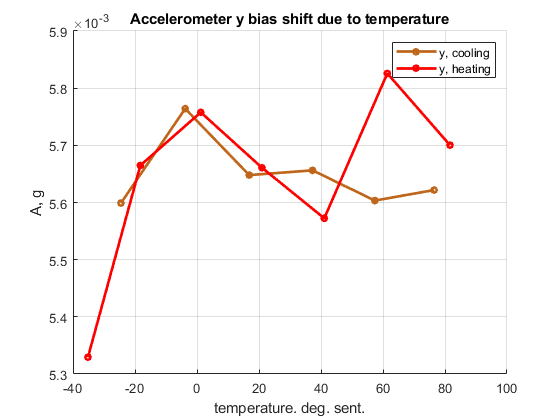
\includegraphics[width=0.9\textwidth]{Ay_accel.png} 
\caption{\label{fig:Ay_accel} Смещения нуля оси Y акселерометра в температуре.}
\end{figure}
\begin{figure}
\centering
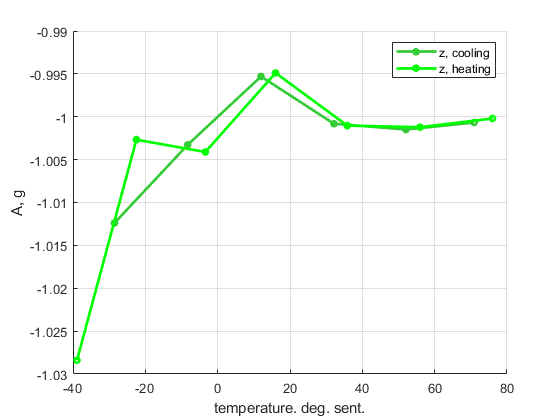
\includegraphics[width=0.9\textwidth]{Az_accel.png} 
\caption{\label{fig:Az_accel} Смещения нуля оси Z акселерометра в температуре.}
\end{figure}

\subsection{Оценка ошибки смещения нуля при непрерывном изменении температуры}

Результаты проведения четырёх экспериментов при непрерывном повышении температуры с -40 до 90 градусов представлены на рисунке ~\ref{fig:four_exps}. В данных экспериментах нагрев проводился с разными скоростями (2 $^{\circ}$C/мин и 5 $^{\circ}$C/мин). Как видно из рисунка, сдвиг нуля гиросокопа имеет сильную повторяемость и не зависит от скорости нагрева прибора, однако при охлаждении датчика присутствует существенный гистерезис. На рисунке ~\ref{fig:hyst} представлен один из экспериментов охлаждения с последующим нагревом. Как видно, на графике у всех осей есть значительный гистерезис.

\begin{figure}
\centering
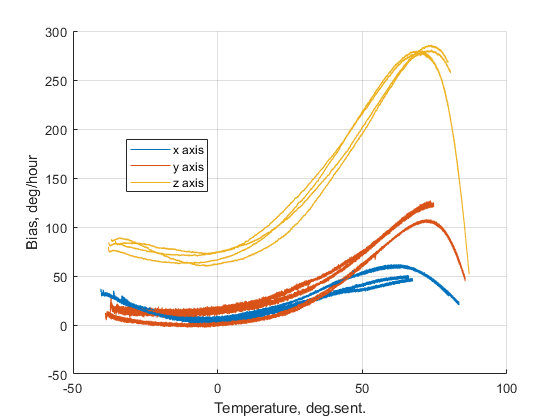
\includegraphics[width=0.9\textwidth]{four_graphs.png} 
\caption{\label{fig:four_exps} Смещения нуля гироскопов при повышении температуры. Четыре эксперимента.}
\end{figure}
\begin{figure}
\centering
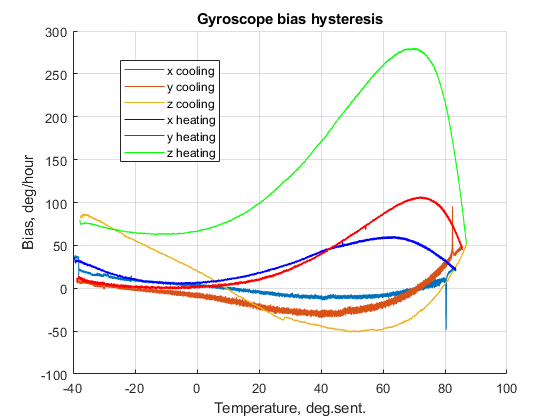
\includegraphics[width=0.9\textwidth]{hysteresis.png} 
\caption{\label{fig:hyst} Гистерезис угловой скорости (точка изменения - слева. Охлаждение сменяется нагревом.}
\end{figure}

Для нахождения скорости ухода смещения нуля за один градус цельсия была посчитана производная от смещения нуля в температуре. Типичный график представлен на рисунке  ~\ref{fig:gradi}. Как видно из графиков, изменение смещения нуля может достигать 1-2 градусов в час на градус цельсия для осей $X$ и $Y$ и 4 градусов в час на градус цельсия для  оси $Z$.

\begin{figure}
\centering
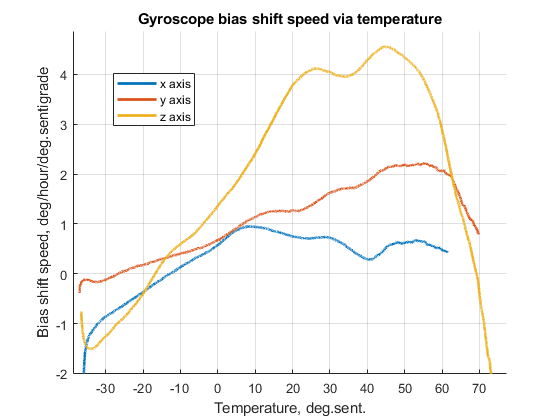
\includegraphics[width=0.9\textwidth]{gradient_labeled.png} 
\caption{\label{fig:gradi} Скорость изменения смещения нуля гироскопа от температуры, $^{\circ}/h/^{\circ}C$ .}
\end{figure}

На рисунках ~\ref{fig:accX_hyst} и ~\ref{fig:accY_hyst} преведены графики смещения нулей в температуре для осей $X$ и $Y$ акселерометра.

\begin{figure}
\centering
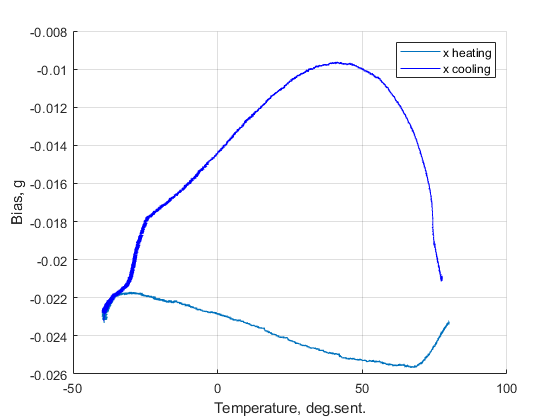
\includegraphics[width=0.9\textwidth]{AccX_hyst.png} 
\caption{\label{fig:accX_hyst} Смещение нуля в температуре. Акселерометр. Ось Х.}
\end{figure}

\begin{figure}
\centering
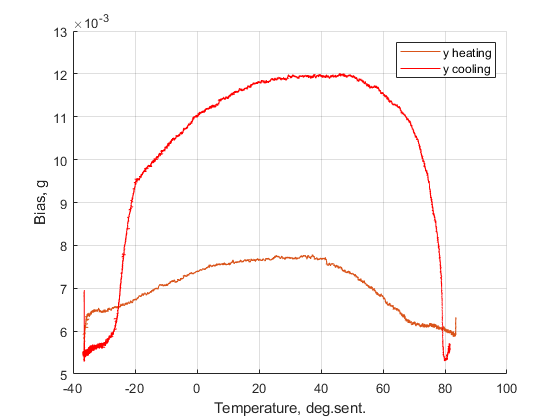
\includegraphics[width=0.9\textwidth]{AccY_hyst.png} 
\caption{\label{fig:accY_hyst}  Смещение нуля в температуре. Акселерометр. Ось Y.}
\end{figure}


\subsection{Оценка ошибки смещения нуля и масштабного коэффициента на одной температурой точке на поворотном столе}
Для оценки ошибок смещения нуля акселерометров были проведены следующие эксперименты: на поворотном столе в комнатной температуре прибор МГ-25 был повёрнут в 26 различных положений. В каждом положении по показаниям поворотного стола были вычислены истинные ускорения, которые затем были вычтены из действительных показаний прибора МГ-25. Получившиеся ошибки показаны на рисунке  ~\ref{fig:accel_biases}. На рисунке  ~\ref{fig:accelscale} показаны те же ошибки, зависящие от ускорения, измеряемого данной осью в данном положении.

\begin{figure}
\centering
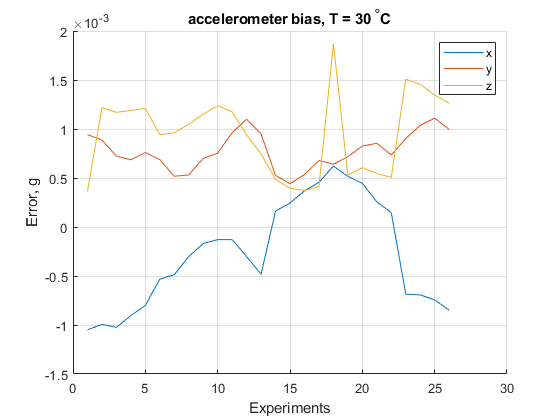
\includegraphics[width=0.9\textwidth]{accel_biases.png} 
\caption{\label{fig:accel_biases}  Смещение нуля акселерометра в разных положениях.}
\end{figure}

\begin{figure}
\centering
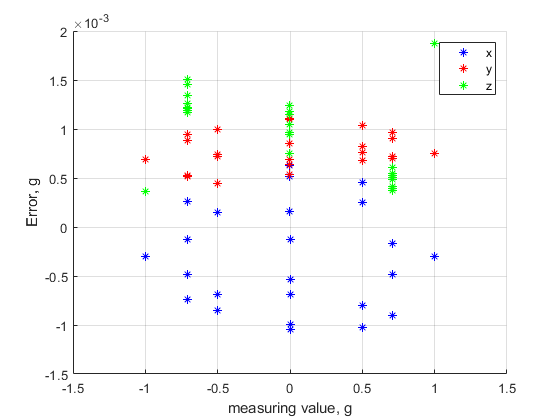
\includegraphics[width=0.9\textwidth]{accelscale.png} 
\caption{\label{fig:accelscale}   Смещение нуля акселерометра от измеренного осью ускорения.}
\end{figure}

Для гироскопов были проведены аналогичные эксперименты: 26 статических положений, 26 положений при вращении внешней оси поворотника со скоростью 30 $^{\circ}$/с и по 4 положения с вращением вокруг оси $Z$ со скоростями $\pm$60, $\pm$120 и $\pm$180 30 $^{\circ}$/с. Полученные результаты показаны на рисунке ~\ref{fig:gyros_errors}. Из-за не идеальности калибровки на скоростях $\pm$60, $\pm$120 и $\pm$180 30 $^{\circ}$/с ось $Y$ измеряет значительную проекцию вращения. Те же данные, зависящие от измеряемого значения угловой скорости представлены на рисунке ~\ref{fig:gyros_errors_dots}.

\begin{figure}
\centering
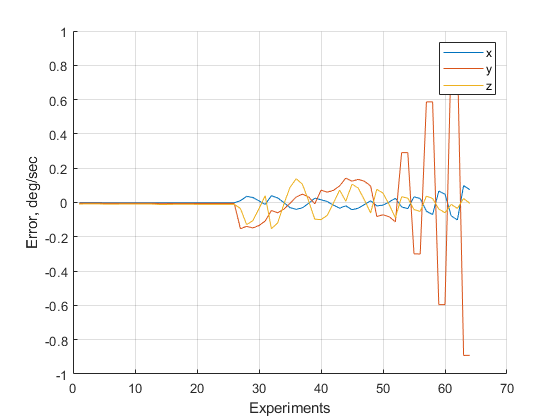
\includegraphics[width=0.9\textwidth]{gyros_errors.png} 
\caption{\label{fig:gyros_errors}  Смещение нуля гироскопов в разных положениях.}
\end{figure}

\begin{figure}
\centering
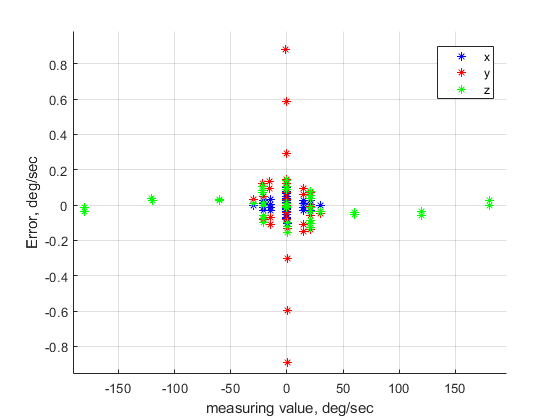
\includegraphics[width=0.9\textwidth]{gyros_errors_dots.png} 
\caption{\label{fig:gyros_errors_dots}   Смещение нуля гироскопов от измеренного осью ускорения.}
\end{figure}



\section{Гирокомпасирование}
В данной работе под "углом места" подразумевается угол между осью Z прибора МГ-25 и вертикальной осью. То есть, если угол места равен 90 градусам, это означает, что датчик расположен горизонтально.
\subsection{Приведение системы координат МГ-25 к оси вращения.}

Для правильной работы алгоритма требуется привести оси (акселерометра и гироскопа) к внутренней оси вращения системы. Для этого требуется поставить прибор МГ-25 в вертикальное положение (ось Z акселерометра вверх) и провести следующие процедуры: снять и усреднить показания акселерометра по оси $x$ (обозначим как $ax_1$) и y (обозначим как $ay_1$) в течение нескольких секунд, затем повернуть МГ-25 на 180 градусов внутренним двигателем и таким же образом ещё раз снять усреднённые показания осей х и у ($ax_2$ и $ay_2$).   \textcolor{red}{ Важно, чтобы остальная конструкция системы оставалась неподвижной во время всей процедуры.}



Для нахождения матрицы доворота используются следующие выражения\footnote{Для малых углов отклонения системы от вертикали (не более 7 градусов) можно использовать упрощенные формулы нахождения углов: $\alpha = \frac{ax_1+ax_2}{2}$ и $\beta = - \frac{ay_1+ay_2}{2}$, которые дадут дадут дополнительную ошибку определения угла места не более 0.01 градуса. }:

\[ \alpha = \frac{arcsin(ax_1)+arcsin(ax_2)}{2}\]
\[ \beta = - \frac{arcsin(ay_1)+arcsin(ay_2)}{2}\]

\[
R = 
\begin{bmatrix}
cos(\alpha) & 0 & -sin(\alpha)\\
sin(\alpha)sin(\beta) & cos(\beta) & cos(\alpha)sin(\beta) \\
cos(\beta)sin(\alpha) & -sin(\beta) & cos(\alpha)cos(\beta)
\end{bmatrix}
\]

Если используется MatLab, $R = angle2dcm(0, \alpha, \beta)$.

Все получаемые в дальнейшем значения акселерометров и гироскопов нужно предварительно домножить на матрицу $R$

\subsection{Проведенные эксперименты и результаты.}

Для исследования точности определения азимута прибором МГ-25, он был закреплён на трехосевом поворотном столе, внешняя ось поворотного стола задавала истинный угол азимута, вторая ось поворотного стола задавала угол места, третья ось - четыре поворота вокруг оси $Z$ прибора с шагом 90 градусов. Всего было снято 25 различных положений с разными углами азимута и места (Азимут - 0, 12, 90, 180 и 270 относительно севера, угол места - 1, 10, 20, 34, 56 градусов относительно вертикали). Эксперименты были проведены в комнатной температуре с предварительным ожиданием стабилизации температуры в приборе. В каждой точке, ипользуя показания акселерометров, вычисляется угол места прибора и затем по полученной проекции вектора вращения земли и вектора ускорения свободного падения на плоскость $XY$ датчика вычисляется угол азимута. В каждом положении датчик снимал показания 2 минуты за оборот (по 30 секунд на каждый оборот внутренней оси 0, 90, 180 И 270 градусов). Весь эксперимент был повторён 4 раза подряд для каждого положения, полученные ошибки усреднены по четырем точкам.

Зная истинное положение датчика по поворотному столу и получая значения угла места и азимута от прибора МГ-25 мы можем получить ошибки определения угла места и азимута. Типичный график ошибок для проведенных экспериментов представлен на рисунках ~\ref{fig:Azim} \footnote{В каждом положении мы вращаем датчик на 90 градусов, тем самым снимая показания двумя осями Х и У со всех четырёх сторон и находим по ним угол азимута. Однако, в реальных условиях иногда возможно вращать прибор только на 180 градусов. Для вычисления азимута в этом случае используется одна часть данных с оси Х и другая часть данных с перпендикулярной оси У. Таким образом мы имеем все направления и можем посчитать проекцию вектора угловой скорости земли только по одному повороту на 180 при помощи двух осей. Из-за большего числа поворотов в ходе эксперимента мы можем комбинировать оси Х и У двумя способами, что и отображено на графике. } и ~\ref{fig:Elev} . По оси х отложены разные положения прибора, упорядоченные по уменьшению угла места (у первых пяти точек угол места равняется 56 градусам, у последних - 1 градусу).

\begin{figure}[h] 
\centering
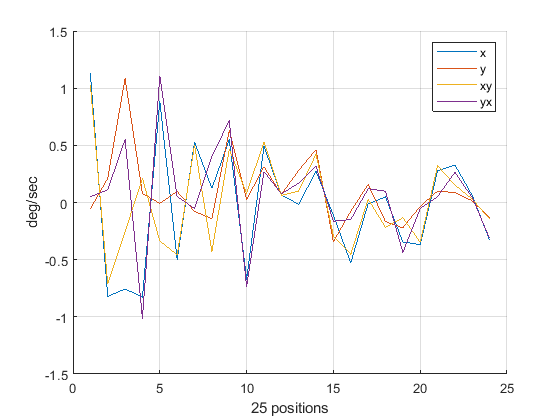
\includegraphics[width=0.9\textwidth]{Azim_err.png} 
\caption{\label{fig:Azim} Ошибка нахождения угла азимута.}
\end{figure}

\begin{figure}[h] 
\centering
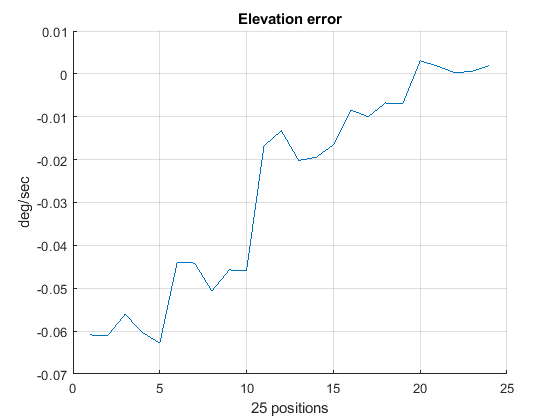
\includegraphics[width=0.9\textwidth]{Elev_err.png} 
\caption{\label{fig:Elev} Ошибка нахождения угла места.}
\end{figure}

Было проведено исследование на влияние количества измерений и длительности измерения в одном положении с дальнейшим усреднением данных на ошибку угла азимута для оценки времени, требуемого для измерения угла азимута с требуемой точностью. Исходные данные (4 повторения эксперимента с 4-мя поворотами на 90 градусов каждой оси с ожиданием в 30 секунд в каждой точке) были разделены по 10,20 и 30 секунд ожидания в каждой точке и усреднением результатов по 1,2,3 или 4 повторениям (рис ~\ref{fig:Matrix}, красным помечено общее время, необходимое для измерения).  Для каждой точки в получившейся сетке были посчитаны ошибки нахождения угла азимута и построены поверхности ошибок по исходной сетке. Пример поверхности для максимальной ошибки оси Х представлен на рисунке ~\ref{fig:Mesh}. 
\begin{figure}[h] 
\centering
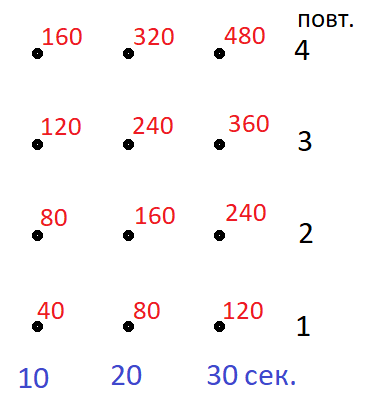
\includegraphics[width=0.4\textwidth]{matrix.png} 
\caption{\label{fig:Matrix} Исходная сетка.}
\end{figure}

\begin{figure}[h] 
\centering
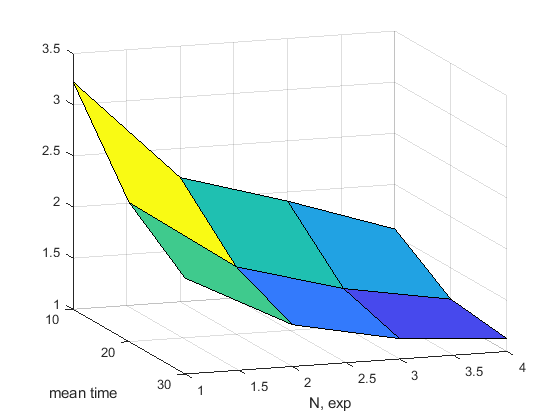
\includegraphics[width=0.9\textwidth]{mesh.png} 
\caption{\label{fig:Mesh} Максимальная ошибка оси Х.}
\end{figure}

Целью построения таких поверхностей было определение оптимальной стратегии измерения угла азимута - лучше ли за определённое время делать больше измерений либо же просто дольше ждать и усреднять по большему интервалу времени. Из полученных графиков следует, что при стабильной температуре внутри прибора нет разницы между тем, каким образом вести измерения, точность измерения зависит лишь от самого общего времени, затраченного на измерения. Далее приведены графики максимальной (~\ref{fig:err_max}) и средней (~\ref{fig:err_mean}) ошибки измерения угла азимута от времени, затраченного на измерения.

\begin{figure}[h] 
\centering
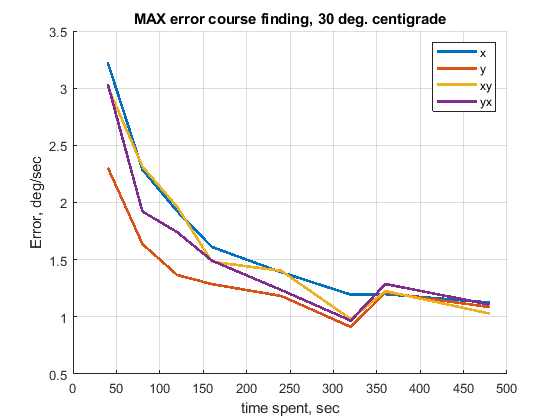
\includegraphics[width=0.9\textwidth]{err_max.png} 
\caption{\label{fig:err_max} Максимальная ошибка определения угла азимута от времени.}
\end{figure}

\begin{figure}[h] 
\centering
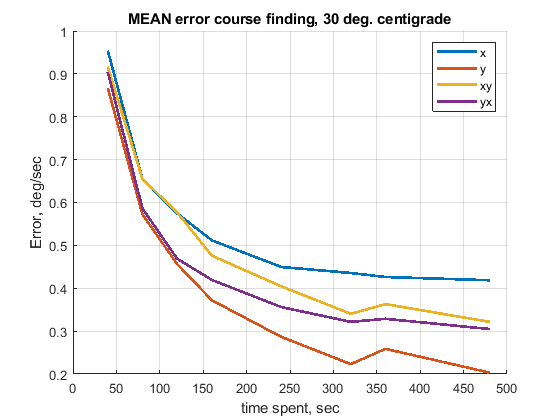
\includegraphics[width=0.9\textwidth]{mean_err.png} 
\caption{\label{fig:err_mean} Средняя ошибка определения угла азимута от времени..}
\end{figure}




\end{document}